\section{Case Study}
\label{sec:av_case_study}

An Autonomous vehicle is a perfect example of a safety critical system that can be deisgned using the compositional techniques discussed in this thesis. The system is composed of multiple components that interact with each other to achieve a common goal, i.e. the goal of driving safely on the road. Usually, the system is also composed of multiple sensors that provide information about the environment (the road conditions and the driving conditions), and multiple actuators that allow the system to interact with the environment. The system is also composed of multiple controllers that are responsible for making decisions about how to interact with the environment. 


\subsection{Road Layout}
\begin{figure}[htbp]
    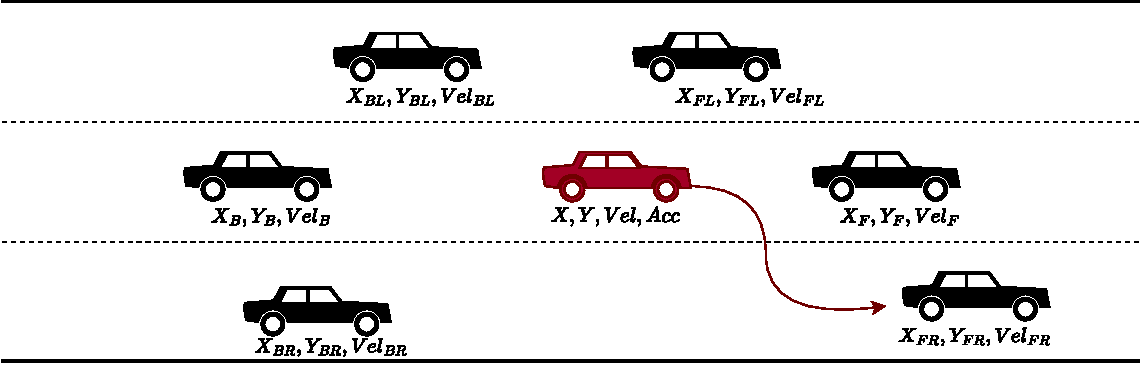
\includegraphics[width=\textwidth]{sections/av/fig/Car_Placement.pdf}
    \caption{General car placement on a freeway}
    \label{fig:car_placement}
\end{figure}

Consider the car placement on a freeway as shown in Figure \ref{fig:car_placement}. This will be the default car placement for this case study. Specifically, the red car is the subject vehicle and it is surrounded by six other cars at any time - two in either lanes and one in front and one at back. If any of the surrounding cars are missing, an imaginary car at the edge of the sensor range is considered. 

Figure \ref{fig:av} shows the various modules that control the behaviour of the subject vehicle. We do not consider any specific sensors in this work, but assume that the car has sensors adequate to provide the information required for the AV to make decisions. This is accounted for by the Perception module. The LCD module is responsible for deciding when it is safe to change lanes. The CF and LCE modules are mathematical models that control the car following behaviour, lane change execution, and obstacle avoidance, respectively. The CF module is responsible for maintaining a safe distance from the car in front. The LCE module is responsible for executing the lane change. The controller module controls changes in the car behaviour by choosing which module outputs should be sent to the car controls.

\begin{figure}[H]
    \centering
    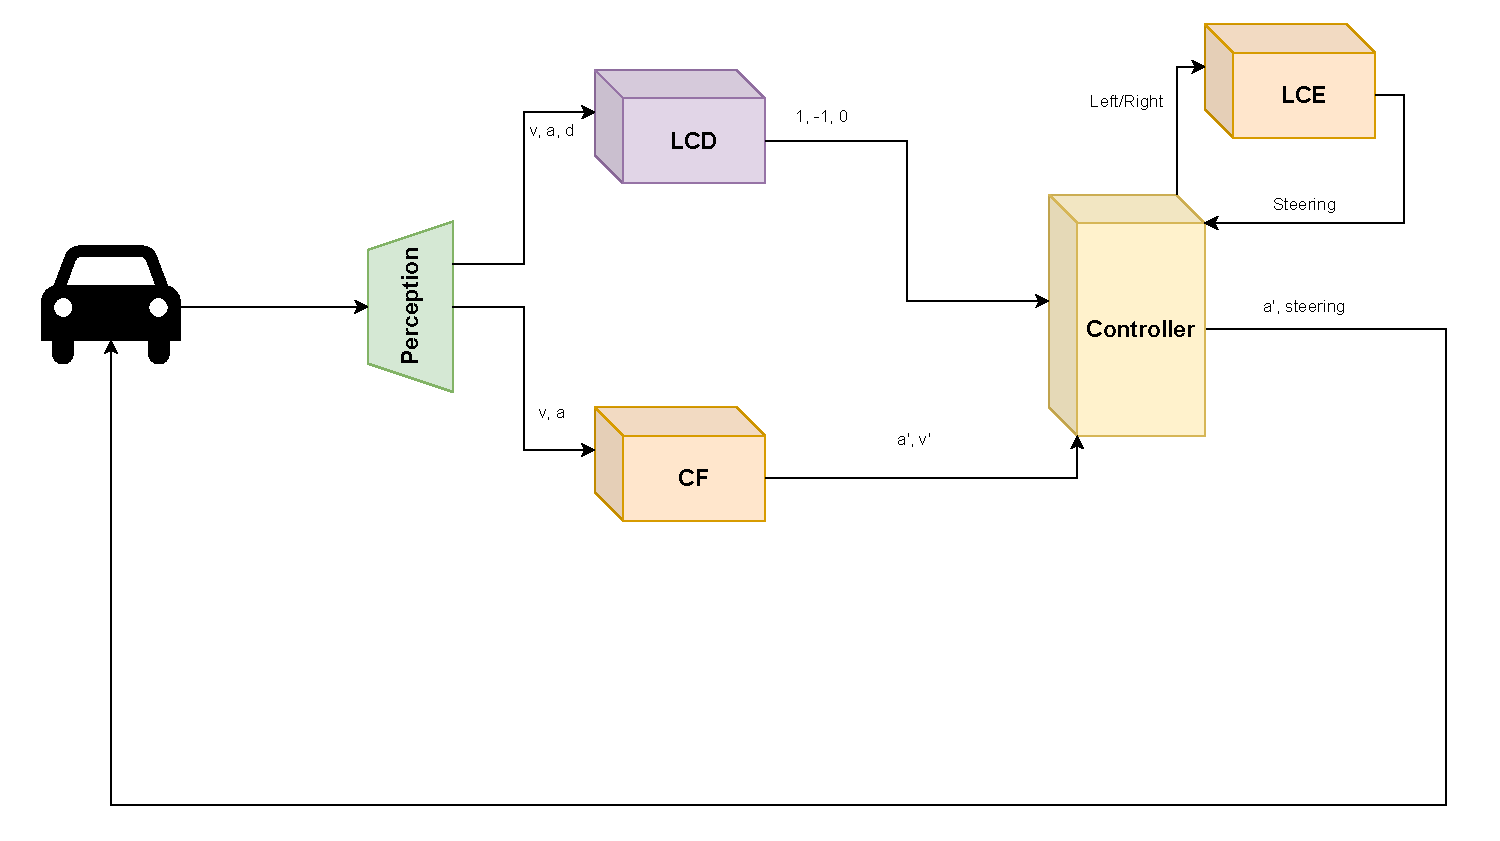
\includegraphics[width=\textwidth]{sections/av/fig/AV_full.pdf}
    \caption{AV case study}
    \label{fig:av}
\end{figure}

\subsection{Car Following Module}
We use the Intelligent Driver Model (IDM) model for Car Following (CF). The IDM model is a car-following model that describes the dynamics of a vehicle following another vehicle. The model is based on the assumption that the vehicle follows the vehicle in front by maintaining a safe distance. The model is given by the following equation:

\begin{equation}
    \begin{aligned}
        \dot{v} &= a \left( 1 - \left( \frac{v}{v_0} \right)^\delta - \left( \frac{s^*}{s} \right)^2 \right) \\
        \dot{s} &= v
    \end{aligned}
\end{equation}

where $v$ is the velocity of the vehicle, $s$ is the distance between the vehicle and the vehicle in front, $a$ is the acceleration, $v_0$ is the desired velocity, $\delta$ is the acceleration exponent, and $s^*$ is the desired safe distance. We choose $v_0 = 30 m/s$ and $s^* = 2m$. IDM model is used in this work for its simplicity and its ability to include driver preferences in modelling car-following behaviour.



\subsection{Lane Change Decision Module}
The Lane Change Decision (LCD) ANN model is responsible for deciding when it is opportune and safe to change lanes. It is a compositional ANN module with three stages as shown in Figure \ref{fig:3_stage_decomposition}. The module contains three ANN models and two \emph{merge} blocks. The Left and Right Safety ANN models are responsible for deciding if it is safe to change lanes to the left or right, respectively. The Merge block combines the outputs of the Left and Right Safety ANN models to decide if it is safe to change lanes. The Opprtunity block is responsible for deciding if it is opportune to change lanes. The merge block combines the outputs of the Safety and Opportunity blocks to decide if it is safe and opportune to change lanes.

\begin{figure}
    \centering
    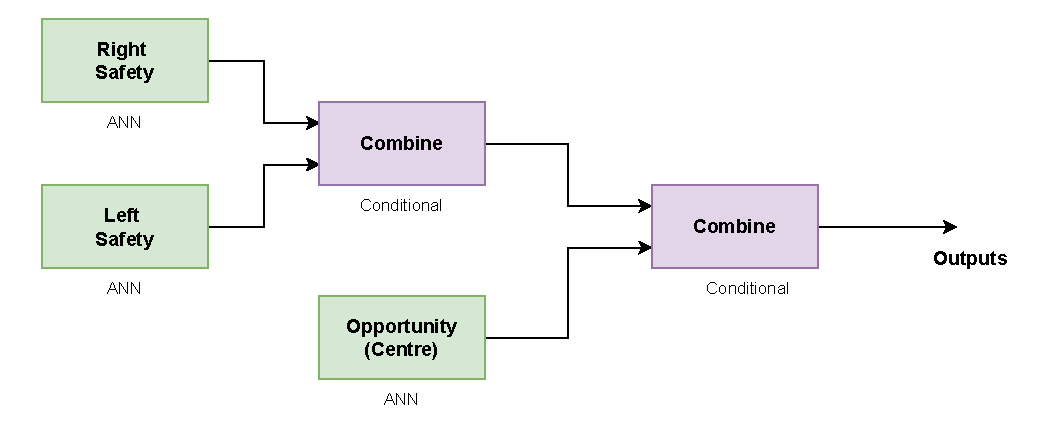
\includegraphics[width=\textwidth]{sections/av/fig/PropertiesComp.pdf}
    \caption{3-stage decomposition of the Lane Change Decision Module}
    \label{fig:3_stage_decomposition}
\end{figure}

To elaborate further, the Left Safety model takes the left and centre lane car states as inputs, namely, the velocity, acceleration, positions of the five cars (including the subject vehicle) in the left and centre lanes. We also consider the maximum desired velocity of the subject vehicle to consider lane change incentive. Similarly, the Right Safety model takes the right and centre lane car states as inputs. The Opportunity model takes the velocity, acceleration, position, and lane of the cars in the centre lane only as inputs. All three models output a binary variable (0 or 1) as output indicating whether the car should lane change or not. While the first merge block also outputs a binary decision, the final merge block outputs -1, 1, or 0, indicating whether the car should lane change to the left, right or stay in the exiting lane, respectively.

\subsubsection{HighD Dataset}
This study uses the highD trajectory dataset recorded by drones at six different Germany highways (\cite{}) to build the models for the LCD module. The dataset contains 60 recordings over 16.5 hours from six locations (labelled 1–6) at different times of the day, covering various density of traffic flows, at a frame frequency of 25Hz. The vehicle trajectories were recorded on highways with either no speed limit or with a limit of 120 km/h and 130 km/h. The typical speeds for trucks and cars at the recording sites are 80 km/h and 120 km/h, respectively. The vehicles (81\% cars and 19\% trucks) in the dataset travel a total of 45,000km, with 11,000 lane changes and 5,600 complete lane changes \cite{}. Several algorithms and post-processing were applied on the raw trajectory data to retrieve smooth position, velocities, and accelerations in both x and y direc- tions, and information, such as the lane number, the time and space headway among others, about the vehicle trajectories.

The car and truck speeds in highD are closer to the actual highway traffic flow and are much higher than those in the much widely used NGSIM dataset \cite{administration_next_2016}. Moreover, the highD dataset includes more than 11,000 lane changes, which is twice the number of NGSIM. Furthermore, the highD dataset has a higher quality of data than NGSIM. Specifically, the NGSIM dataset is coarser with samples collected at 10 Hz, and it includes many errors in the trajectory of the vehicles performing lane changes \cite{}. This affects the model parameters and the ability of the model to generalise to actual scenarios. Therefore, we choose the highD dataset for our developing and testing our approach.


\subsection{Lane Change Execution Model}
The LCE model is a simple polynomial model that describes the lateral position of the vehicle during a lane change. The model is based on the assumption that the vehicle changes lanes by following a polynomial trajectory. The lateral velocity is computed by taking the derivative of the polynomial that describes the lateral position. The model is given by the following equation:

\begin{multline}
    y(t) = a_3 t^3 + a_2 t^2 + a_1 t + a_0\\
    \dot{y}(t) = 3a_3 t^2 + 2a_2 t + a_1\\
    a1 = 0, a2 = 0, a3 = 3 \frac{lane\_width}{t_{LC}^2}, a4 = -2 \frac{lane\_width}{t_{LC}^3}
\end{multline}

where $y(t)$ is the lateral position of the vehicle at time $t$, $a_3$, $a_2$, $a_1$, and $a_0$ are the polynomial coefficients, and $t$ is the time. $t_{LC}$ is the desired time for lane change. Here, $t_{LC} = 5 seconds$ and $lane\_width = 3.7 m$. The model is used in this work for its simplicity and its ability to describe the lateral position of the vehicle during a lane change.



\subsection{Controller Module}


\begin{figure}[htbp]
    \centering
    \begin{tikzpicture}[->,shorten >=1pt,auto,node distance=3.5cm,
        el/.style = {inner sep=2pt, align=left, sloped},
        every label/.append style = {font=\small},semithick,initial where=left]

        \tikzstyle{every node}=[font=\small]
        \tikzstyle{state}=[circle,thick,draw=blue!75,fill=blue!20,minimum size=10mm]
        \tikzstyle{transition}=[align=center]

        % Nodes
        \node[initial,state] (CF) at (0,0) {CF};
        \node[state] (Wait) at (3.5,5) {Wait};
        \node[state] (LC) at (7,0) {LCE};

        % Transitions
        \path (CF) edge[loop below] node[transition] {LCD = 0} (CF)
              (CF) edge node[transition] {LCD = $\pm$1; t $=$ 0} (Wait)
              (Wait) edge[loop above] node[transition] {t $\leq$ 1\\LCD = $\pm$1} (Wait)
              (Wait) edge node[transition] {LCD $\land$ t $>$ 1; LCE = 1} (LC)
              (Wait) edge[bend left] node[transition] {LCD = 0} (CF)
              (LC) edge[loop below] node[transition] {LCE=1} (LC)
              (LC) edge node[transition] {LCE=0} (CF);

    \end{tikzpicture}
    \caption{A finite state model diagram for the AV controller. Each state represents a phase of operation, and transitions are defined by the conditions derived from inputs and internal counters.}
    \label{fig:av_controller}
\end{figure}



The finite state diagram shown in Figure~\ref{fig:av_controller} illustrates the operation of the Autonomous Vehicle (AV) controller. The controller switches between three primary states: \textbf{Car Following (CF)}, \textbf{Waiting (Wait)}, and \textbf{Lane Change Execution (LCE)}. Each state corresponds to a phase in the operation, and transitions between these states are governed by specific conditions derived from inputs, time variables, and internal counters.

The system begins in the \textbf{Car Following (CF)} state. While in this state, the controller remains in CF as long as the Lane Change Decision (LCD) signal is zero, indicating no decision to perform a lane change. However, when an LCD signal of $\pm1$ (indicating a left or right lane change decision) is received, and the timer $t = 0$, the system transitions to the \textbf{Waiting (Wait)} state. This transition initiates a temporary state where the lane change decision is further evaluated.

In the \textbf{Waiting (Wait)} state, the controller assesses whether the LCD signal persists and the timer $t \leq 1$ second, which keeps the system in the same state. This delay helps ensure that transient LCD signals do not cause premature lane change execution. If the LCD signal continues and the timer surpasses a threshold value of $1$ second (10 steps at 10 Hertz sampling rate), the controller activates Lane Change Execution (LCE) by transitioning to the \textbf{Lane Change Execution (LCE)} state. Conversely, if the LCD signal returns to zero during the Waiting state, the system transitions back to the \textbf{Car Following (CF)} state, aborting the lane change decision.

In the \textbf{Lane Change Execution (LCE)} state, the controller actively performs a lane change. It remains in this state as long as the LCE signal is set to $1$, signifying that the execution is ongoing. Once the LCE signal switches to $0$, indicating the completion of the lane change, the controller transitions back to the \textbf{Car Following (CF)} state, resuming its default behaviour.


